\graphicspath{{chapters/15/}}
\chapter{Evolutionary Trees from DNA Sequences: A Maximum Likelihood Approach}
\section{Maximum likelihood estimation}
In statistics, maximum likelihood estimation (MLE) is a method of estimating the parameters of an assumed probability distribution, given some observed data. This is achieved by maximizing a likelihood function so that, under the assumed statistical model, the observed data is most probable. The point in the parameter space that maximizes the likelihood function is called the maximum likelihood estimate.
\subsection{Principles}
We model a set of observations as a random sample from an unknown joint probability distribution which is expressed in terms of a set of parameters. The goal of maximum likelihood estimation is to determine the parameters for which the observed data have the highest joint probability. We write the parameters governing the joint distribution as a vector ector 
$\;\theta =\left[\theta _{1},\,\theta _{2},\,\ldots ,\,\theta _{k}\right]^{\mathsf {T}}\;$
so that this distribution falls within a parametric family 
$\;\{f(\cdot \,;\theta )\mid \theta \in \Theta \}\;$ where $\Theta$ is called the parameter space, a finite-dimensional subset of Euclidean space.
Evaluating the joint density at the observed data sample 
$ \;\mathbf {y} =(y_{1},y_{2},\ldots ,y_{n})\;$
gives a real-valued function,

\begin{equation}
{\mathcal {L}}_{n}(\theta )={\mathcal {L}}_{n}(\theta ;\mathbf {y} )=f_{n}(\mathbf {y} ;\theta )\;
\end{equation}

which is called the likelihood function. For independent and identically distributed random variables, $ f_{n}(\mathbf {y} ;\theta $
will be the product of univariate density functions:

\begin{equation}
{\displaystyle f_{n}(\mathbf {y} ;\theta )=\prod _{k=1}^{n}\,f_{k}^{\mathsf {univar}}(y_{k};\theta )~.}
\end{equation}

The goal of maximum likelihood estimation is to find the values of the model parameters that maximize the likelihood function over the parameter space,[6] that is

\begin{equation}
{\hat {\theta }}={\underset {\theta \in \Theta }{\operatorname {arg\;max} }\,{\mathcal {L}}_{n}(\theta \,;\mathbf {y} )~.}
\end{equation}

Intuitively, this selects the parameter values that make the observed data most probable. The specific value 
$  ~{\hat {\theta }}={\hat {\theta }}_{n}(\mathbf {y} )\in \Theta $ that maximizes the likelihood function 
$ \,{\mathcal {L}}_{n}\,$ is called the maximum likelihood estimate. Further, if the function 
$ \;{\hat {\theta }}_{n}:\mathbb {R} ^{n}\to \Theta \;$
so defined is measurable, then it is called the maximum likelihood estimator. It is generally a function defined over the sample space, i.e. taking a given sample as its argument. A sufficient but not necessary condition for its existence is for the likelihood function to be continuous over a parameter space $\Theta$ that is compact.[7] For an open $\Theta$  the likelihood function may increase without ever reaching a supremum value.
In practice, it is often convenient to work with the natural logarithm of the likelihood function, called the log-likelihood:
\begin{equation}
\ell (\theta \,;\mathbf {y} )=\ln {\mathcal {L}}_{n}(\theta \,;\mathbf {y} )~.
\end{equation}

\subsection{Phylosophy}
The maximum likelihood method finds that estimate of a parameter which maximizes the probability of observing the data given a specific model for the data.\\
Likelihood principle: “In statistics, the likelihood principle is the proposition that, given a statistical model, all the evidence in a sample relevant to model parameters is contained in the likelihood function.” 

\subsection{ML for phylogenetic trees}
Given a multiple sequence alignment and probabilistic model of for substitutions (like PAM does, but different) find the tree which has the highest probability of generating the data. 
\\
It was first proposed by Felsestein in 1981, assuming some simplifying assumptions:
\begin{itemize}
\item Positions evolved independently
\item After species diverged they evolve independently
\end{itemize}

Formally, the task of the algorithm is to find the tree T such that assuming evolution model M $Pr[Data| T,M]$ is maximized.

\section{Introduction}
Problem with parsimony methods is that they implicitly assume that change is improbable a priori. If the amount of change is small over the evolutionary times being considered, parsimony methods will be well-justified statistical methods.
Most data however involve moderate to large amounts of change, and it is in such cases that parsimony methods can fail.
\\
Distance approaches estimate the tree from information on the pairwise similarity of the sequences (Fitch and Margoliash 1967), without attempting to make full use of the information available in the original sequences.

\section{Computing likelihood of a tree }
Maximum likelihood estimation is the method of statistical inference most readily applicable to data of this sort. It involves finding that evolutionary tree which yields the highest probability of evolving the observed data. 
Note that although the likelihood of a tree is the probability of the data given the hypothesis, it is taken as a function of the hypothesis (the tree) rather than a function of the data. This means that the likelihoods for different trees do not sum to unity.
Note also that the likelihood of a tree is not the probability that the tree is the correct one.
\\
The problem reduces to computing the probability of a particular set of sequences on a given tree and maximizing this probability over all evolutionary trees.
The assumption of independent events, even if not biologically correct, makes the computation feasible. 
Since we are willing to assume independence of evolution at different sites, it turns out that the probability of a given set of data arising on a given tree can be computed site by site, and the product of the probabilities taken across sites at the end of the computation.
\\
So we concentrate on computing this probability for a single site. 
For this we make use of the probabilities $Pij(t)$, where $i$ and $j$ take values 1,2, 3, and 4 corresponding to the four bases A, C, G, and T. $Pij(t)$ is the probability that a lineage which is initially in state $i$ will be in state $j$ after $t$ units of time have elapsed. We compute the $Pij(t)$ later, for the moment
we concentrate on obtaining an expression for the likelihood of the tree.
\\
We assume that after speciation two lineages evolve independently, and that the same stochastic process of base substitution applies in all lineages.
Instead of writing general expression for the likelihood of a tree, we will refer to a specific case, shown in figure \ref{fig:tree1}.

\begin{figure}[H]
		\centering
		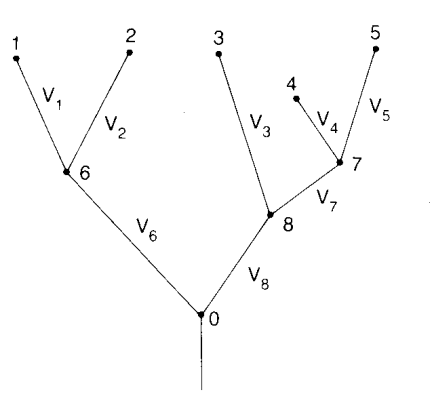
\includegraphics[width=0.5\textwidth]{tree1.png}
		\caption{The tree used in the discussion of computing the likelihood. The v's are the lengths of the segments }
		\label{fig:tree1}
	\end{figure}

The lengths of the segments of the tree are given by $v_i$. If we knew the states (bases) at a particular site at points 0, 6, 7 and 8 on this tree, and these were $s_0$, $s_6$, $s_7$, and $s_8$, the likelihood of the tree would be the product of
the probabilities of change in each tree segment, times the prior probability $\pi_{s_0}$ of state $s_0$. In practice we do not know $s_0$, $s_6$, $s_7$, and $s_8$, so the likelihood will be the sum over all possible assignments of bases to those forks on the tree:

\begin{equation}
L = \sum_{s_0} \sum_{s_6} \sum_{s_7} \sum_{s_8} \, \pi_{s_0} \, P_{s_0 s_6}(v_6) \, P_{s_6 s_1}(v_1) \, P_{s_6 s_2}(v_2) \, P_{s_0 s_8}(v_8) \, P_{s_8 s_3}(v_3) \, P_{s_8 s_7}(v_7) \, P_{s_7 s_4}(v_4) \, P_{s_7 s_5}(v_5)
\end{equation}

This expression for $n$ species will have $2^{2n -2}$ terms (in this case, 256).
I will deliberately skip all the simplifications of the expression, what's important to know is that we can define $L_s^{(k)}$ as the likelihood based on the data at or above point $k$ on the tree, given that point $k$ is known to have state $s$ for the site under consideration. If point $k$ is a tip, then  $L_s^{(k)}$ will be zero for all $s$ except that actually observed, for which  $L_s^{(k)}$.
We work our way down the tree from the tips (we perform a postorder tree traversal). For point $k$, whose immediate descendants are $i$ and $j$, we can compute for all four values of $s_k$

\begin{equation}
L_s^{(k)} = \big( \sum_{s_i} P_{s_k s_i}(v_i) L_{s_i} ^{(i)} ) (\sum_{s_j} P_{s_k s_j}(v_j) L_{s_j} ^{(j)} \big)
\end{equation}

For the bottom fork, point 0 in our example, we will then have computed the four conditional likelihoods $L_{s_0}^{(0)}$ given the possible states of the site at point 0.

\section{The base substitution probabilities}
We have not yet specified how the quantities $Pij(t)$ are to be computed. These are the probabilities of transition from one base to another over a segment of length $t$. We assume that these probabilities reflect a Markov process, a process in which the probability of a base changing may depend on its current identity, but not on its past history.
\\
We assume that in a small interval of time of length $dt$, there is a probability $u dt$ that the current base at a site is replaced. The quantity u is the rate of base substitution per unit time. 
If a base is replaced, its replacement is A, C, G, or T with probabilities $\pi_1$ $\pi_2$, $\pi_3$, $\pi_4$. Note that this means that a base could be replaced
by the same base, so that not all substitutions are observable even in principle. Note also that this model makes no distinction between transitions and transversions. If we let $delta_{ij}$ be $0$ if $i \neq j$ and 1 if $i = j$ (the
Kronecker delta function), then we are in effect assuming that for infinitesimal $dt$

\begin{equation}
P_{ij}(dt) = (1- u dt) \delta_{ij} + u dt \pi_j
\end{equation}

from this, we can derive 

\begin{equation}\label{eq:7}
P_{ij}(dt) = e^{-ut} \delta_{ij} + (1- e^{-ut}) \pi_j
\end{equation}

This follows almost immediately once one observes that $e^{-ut}$ is the probability that the site does not change at all over a length of time t, and that if it does change the probability that it ends up in state $j$ is $\pi_j$. 

\section{The pulley principle}
The reversibility of our Markov process and the absence of constraints on segment lengths can be used to establish an interesting and useful property of the estimation of evolutionary trees under this model.
Reversibility requires that for all $i$,$j$, and $t$:

\begin{equation}
\pi_i P_{ij}(t) = P_{ji}(t) \pi_j
\end{equation}

Consider the last two steps of our algorithm for calculating likelihoods. 
They involved (in our example) forks 0, 6, and 8 in the expression for the likelihood of the tree at one site.
Since the likelihood L is our only basis for comparing evolutionary trees, this means that the tree whose likelihood is being calculated could have its root anywhere between points 6 and 8, as shown in figure \ref{fig:pulley}a. The root of the tree is a sort of pulley, so that if all parts of the tree to one side of the root are moved down, and all parts to the other side moved up by the same amount, the likelihood remains unaltered.


\begin{figure}[H]
		\centering
		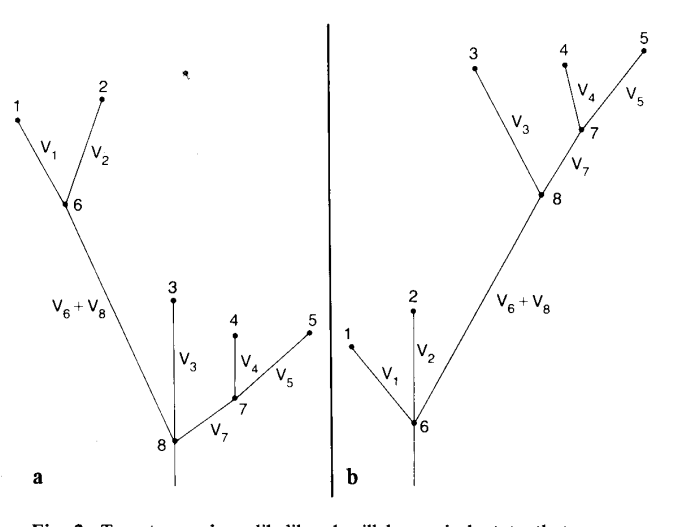
\includegraphics[width=0.5\textwidth]{tree2.png}
		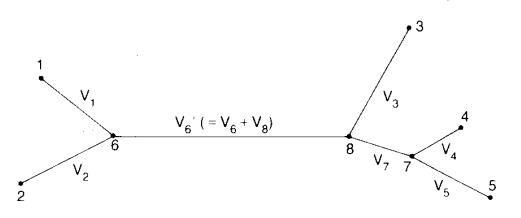
\includegraphics[width=0.5\textwidth]{tree3.png}
		\caption{Visual representation of the pulley principle. (a) Two trees whose likelihood will be equivalent to that in Fig \ref{fig:tree1} under the assumption of this paper (b) The unrooted tree whose likelihood is equivalent to those in Fig \ref{fig:tree1} an \ref{fig:pulley}a }
		\label{fig:pulley}
	\end{figure}


Figure \ref{fig:pulley}b shows the unrooted tree, which is what we are in effect estimating.
The root of the tree can be placed anywhere on that tree without affecting the likelihood.

\section{Finding the Maximum Likelihood tree}
Our interest in the Pulley Principle is that it allows us to regard any given segment of the unrooted tree as contraining the root. This in turn allows us to alter the length of that segment in an optimal fashion, which will be useful.
We have a computationally feasible method for evaluating the likelihood of a given tree, but this leaves us with the task of finding the maximum likelihood tree.
\\
Consider the problem of finding values of the $v_i$ which maximize the likelihood of the tree given a particular topology.
The pulley principle allows us to construct an algorithm which alters one of the $v_i$ at a time, each one being altered to that value which results in the highest likelihood. This process continues until none of the $v_i$ can be altered
in a way which substantially improves the likelihood. At each stage one $v$ is changed to the value which gives the greatest possible likelihood, given that only that $v$ can be varied. Thus at each step the likelihood of the tree increases.

\section{Searching among tree topologies}
There still remains the problem of examining many different tree topologies. 
The strategy proposed is to build the tree up by successively adding species to it, starting with a two-species tree. When the k-th species is being added to the tree, there will be 2k-5 segments from which it could arise. 
Each of these is tried and the maximum likelihood within the resulting topology evaluated, by the iteration technique presented below.
The placement yielding the highest likelihood is accepted.
If the tree now has more than four species, before the next species is added local rearrangements are carried out in the tree to see if any of these improves the likelihood of the tree. 
If any does, it is accepted and the local rearrangement process continues until a tree is found which no local rearrangement can improve.
This strategy of searching among possible topologies is not guaranteed to find the best topology.

\section{Finding optimum segment lengths}
Within each topology we examine, we must adjust the $v_i$ to their maximum likelihood values. 
This is done by adjusting each of the $v_i$ in turn according to a method which guarantees that each of the v i changes to that value which maximizes the likelihood of the tree, given the current values of the other v's.
Consider segment 7 of the tree in figure \ref{fig:pulley}b, the segment connecting nodes 7 and 8. We can consider the root to be located in this segment, and use the pruning algorithm given above to compute the sets of conditional likelihoods at points 7 and 8. Suppose that we take the root to be immediately to the right of point 8. The likelihood of the tree for one site is then given by

\begin{align}\label{eq:10}
L = \sum_{s_0} \sum_{s_6} \sum_{s_7} \sum_{s_8} \, \pi_{s_0} \, (P_{s_0 s_8} L_{s_8}^{(8)}) \, (P_{s_0 s_7}(v_7) L_{s_7}^{(7)}) 
\\
= \sum_{s_0} \pi_{s_0} L_{s_0}^{(8)} ( \sum_{s_7} P_{s_0 s_7}(v_7) L_{s_7}^{(7)}
\end{align}

If we substituite into (\ref{eq:10}) the expression (\ref{eq:7}) with $u=1$, we will obtain an expression that is the factor of the full likelihood which corresponds to one site\footnote{not reported here, it's expression 11 in the original paper}. There is one factor like this for each site in the DNA, so that the full likelihood is of the form

\begin{equation}\label{eq:12}
L = \prod_{i} (A_i q + B_ip)
\end{equation}

where $q= e^{v_7}$, $p= 1-q$ and $A_i$ and $B_i$ are the terms 
\begin{equation}
A_i = \sum_{s} \pi_s L_s ^{(8)} L_s ^{(7)}
\end{equation}

and 
 \begin{equation}
 B_i = (\sum_{s_8} \pi_{s_8} L_{s_8} ^{(8)}) (\sum_{s_7} \pi_{s_7} L_{s_7} ^{(7)})
 \end{equation}

for the i-th DNA site. We want to find the value of $v_7$ which maximizes the likelihood. We can the proceed by taking the logarithm of equation \ref{eq:12} and equating the derivative of this expression to zero. All the steps of this very last part are reported in the paper. 




















